
% Note that there is a condition (line 6 in Pseudocode~\ref{alg:probabilistic model}) to check if there is a valid statistics point.
% This condition is extremely important, because it first provides a basis to distinguish between known facts (i.e., good or bad satisfaction ratio for the incoming interface) and unknown facts (e.g., the first time an Interests arrives on the interfaces).
% Second, it gives an opportunity to recover from a bad history (history of unsatisfied Interests) after malicious Interests are ceased to flow in.
% Essentially, this recovery relies on statistics module to perform time-based invalidation of historical data (timely, but not too quickly\footnote{Otherwise, attackers may send short bursts of malicious Interests, successfully avoiding differential Interest treatment}).


Pseudocode~\ref{algo:interest stats} formally defines per-incoming interface statistics generation.
Please note that in order to ensure decaying of relative statistics (e.g., ratio between the number of unsatisfied and forwarded Interest), only unsatisfied statistics needs to be exponentially smoothed (lines 23--26).  

\floatname{algorithm}{Pseudocode}

%%%%%%%%%%%%%%%%%%%%%%%%%%%%%%
%%%%%%%%%%%%%%%%%%%%%%%%%%%%%%
%%%%%%%%%%%%%%%%%%%%%%%%%%%%%%

\begin{algorithm}[h]
\footnotesize
\caption{\small Interest satisfaction statistics}
\label{algo:interest stats}
\begin{algorithmic}[1]

\vspace{0.2cm}

\For{\textbf{each} interface \em{if}}
    \State $F_{if} \leftarrow 0$ \Comment{forwarded Interests from interface \textbf{if}}
    \State $\hat F_{if} \leftarrow 0$ \Comment{averaged value of $F_{if}$}

    \State $U_{if} \leftarrow 0$ \Comment{unsatisfied Interests from interface \textbf{if}}
    \State $\hat U_{if} \leftarrow 0$ \Comment{averaged value of $U_{if}$}
\EndFor

\vspace{0.2cm}
\Function{OutInterest}{Interest \textbf{i}, InInterface \textbf{if}}
  \State $F_{if} \leftarrow F_{if} + 1$
  \State record \textbf{\emph{if}} in the list of incoming interfaces for \textbf{\emph{i}}
\EndFunction

\vspace{0.2cm}
\Function{InterestTimeout}{Interest \textbf{i}}
    \State lookup the list of incoming interfaces for \textbf{\emph{i}}

    \For{\textbf{each} interface $if$ in the list}
        \State $U_{if} \leftarrow U_{if} + 1$
    \EndFor
\EndFunction

\vspace{0.2cm}

\State {} \Comment{\textit{Exponentially weighted moving average smoothing}}
\Function{EWMA}{} \Comment{Every second}
\State $\alpha \leftarrow e^{-1.0/30.0}$  %\Comment{$\approx$ 30~sec average}

\For{\textbf{each} interface \em{if}}
    \State $\hat U_{if} \leftarrow \alpha \cdot \hat U_{if} + (1 - \alpha) \cdot U_{if}$ 
    \State $U_{if} \leftarrow 0$ 

    \If{$F_{if} > 0$} \Comment{To ensure decaying of ratio $U_{if}/F_{if}$ when Interest flow stops}
        \State $\hat F_{if} \leftarrow \alpha \cdot \hat F_{if} + (1 - \alpha) \cdot I_{if}$ 
        \State $F_{if} \leftarrow 0$ \Comment{Reset counters}
    \EndIf
\EndFor

\EndFunction

\end{algorithmic}
\end{algorithm}


Fig.~\ref{fig:ratio example} illustrates the resulting dynamics of the statistic during (10--70~seconds) and after the attack.
Before the attack started, the percentage of unsatisfied Interests is zero.  
The statistics starts to build up rapidly as soon as Interests start to time out, which happens approximately after one second since the start of the attack.\footnote{Again, we are assuming that Interests are admitted for a maximum period one second.}
For the following duration of the attack, statistics fluctuates near the 100\% mark: 
when the ratio is close to 100\%, routers drop all incoming Interests, resulting in decaying of the statistics until a new Interest is admitted, which eventually brings statistics back near 100\% point.
Finally, the ratio exponentially decays after the attack ceases.

\begin{figure}[htbp]
  \centering
  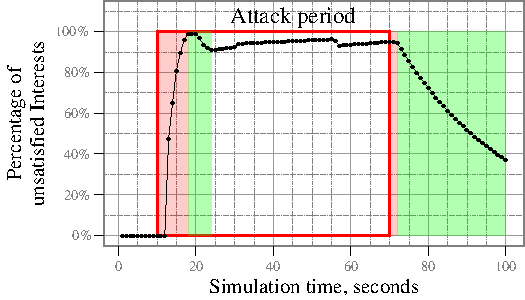
\includegraphics[scale=1]{limits}
  \caption{Dynamics of the unsatisfied Interests statistics on gateway's interface towards the attacker}
  \label{fig:ratio example}
\end{figure}


%%% Local Variables: 
%%% mode: latex
%%% TeX-master: "../paper"
%%% End: 
